\documentclass{llncs}
%\documentclass[letterpaper, 10 pt, conference]{llncs}
%\IEEEoverridecommandlockouts
%\overrideIEEEmargins

\usepackage{cite}
\usepackage{makeidx}
\usepackage[utf8]{inputenc}
%\usepackage[numbers]{natbib}
\usepackage{multirow}
\usepackage{graphicx}
\usepackage[acronym]{glossaries}
\usepackage[usenames,dvipsnames]{color}

%%% For charts%%
\usepackage{tikz}
%\usepackage{verbatim}
%\usepackage[active,tightpage]{preview}
%\PreviewEnvironment{tikzpicture}
%\setlength\PreviewBorder{10pt}%
%%% 

%% For code block %%
\usepackage{listings}
\lstset{basicstyle=\footnotesize\ttfamily,breaklines=true}
\lstset{framextopmargin=0pt,frame=lrbt,rulecolor=\color{Gray}}
%%%

%\usepackage{float}

\newcommand{\apiname}{SAJaS} 
\newcommand{\apilongname}{Simple API for JADE-based Simulations}

%!TEX root = doc.tex

\title{\LARGE \bf
Bridging the Gap between MAS Simulation and Development using a JADE-based API for Repast
}


\author{João Pedro C. Lopes,
	Henrique Lopes Cardoso,
	João S. V. Gonçalves %
}

\institute{
        Department of Informatics Engineering \\
        Artificial Intelligence and Computer Science Laboratory \\
        Faculty of Engineering \\
        University of Porto \\
        Rua Dr. Roberto Frias, 4200-465 Porto, Portugal \\
        \{joao.pedro.lopes, hlc, joao.sa.vinhas\}@fe.up.pt %
}


% Acronym definitions (doesn't render acronyms page)
% format: \newacronym{<label>}{<abbrv>}{<full>}

%% Acronyms and Abreviations

\newacronym{ACL}{ACL}{Agent Communication Language}
\newacronym{AMS}{AMS}{Agent Management System}
\newacronym{AST}{AST}{Abstract Syntax Tree}
\newacronym{ATL}{ATL}{ATLAS Transformation Language}
\newacronym{CeCILL-C}{CeCILL-C}{CEA CNRS INRIA Logiciel Libre (open source license)}
\newacronym{DF}{DF}{Directory Facilitator}
\newacronym{EPL}{EPL}{Eclipse Public License (open source license)}
\newacronym{FIPA}{FIPA}{The Foundation for Intelligent Physical Agents}
\newacronym{FOSS}{FOSS}{Free and Open Source Software}
\newacronym{IDE}{IDE}{Integrated Development Environment}
\newacronym{JADE}{JADE}{Java Agent DEvelopment Framework}
\newacronym{JDT}{JDT}{[Eclipse] Java Development Tools}
\newacronym{MABS}{MABS}{Multi-Agent-Based Simulation}
\newacronym{MAS}{MAS}{Multi-Agent System}
\newacronym{MTS}{MTS}{Message Transport Service}

\newacronym{Repast}{Repast}{Recursive Porous Agent Simulation Toolkit}

\begin{document}


\maketitle
\thispagestyle{empty}
\pagestyle{empty}

%!TEX root = doc.tex

\begin{abstract}

% 1 - Intro
Agent-based applications and simulations are in widespread use today both in research and industry.
\gls{MAS} and \gls{MABS} are two approaches to make use of multi-agent systems technology, each with distinct characteristics and goals.
% 2 - Problem
While open agent-based applications benefit from adopting interaction standards, most \gls{MABS} frameworks do not support them.
% 3 - Proposal 
In this paper we propose an architecture, based on FIPA and JADE, for agent-based simulations, focusing on supporting agent communication using FIPA interaction protocols.
Based on this architecture, we present the \apiname{} API, whose goal is to bring JADE and Repast, two popular \gls{MAS} and \gls{MABS} development frameworks, closer together, facilitating the creation of simulations by JADE programmers and enabling an automatic portability between both tools.
% 4 - Experimentation/Validation
For illustration, we show the creation of a simulation where agents interact in a contract net.
Finally, we present an early overview of a code conversion tool under development, whose aim is to automatically generate a JADE \gls{MAS} from a Repast simulation that makes use of \apiname{}.
% 5 - Conclusions?
%%
%% TODO
%%
\glsresetall
\end{abstract}

%\begin{IEEEkeywords}
%
%\end{IEEEkeywords}


%!TEX root = doc.tex
\section{Introduction} % (fold)
\label{sec:introduction}
%!TEX root = doc.tex
\section{Comparison to Related Work} % (fold)
\label{sec:related_work}

Some works have approached the problem of complementing Repast and JADE's faults by bringing them together in a single framework by means of a middleware. In MISIA \cite{garcia2011misia} and JRep \cite{gormer2011jrep}, the authors' approach was successful in complementing Repast's and JADE's features, allowing them to create Repast simulations that also take advantage of JADE's networking capabilities and use of open standards.

MISIA's approach, as suggested by Figure \ref{fig:misia}, is to use a middle layer that acts as the bridge betweens the two other layers that interact with JADE and Repast S. By extending the representation of Repast and JADE agents and allowing them to communicate internally and to synchronize their state,
they work seamlessly as one.

\begin{figure}[h]
	\centering
	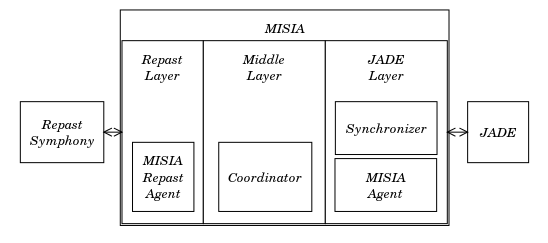
\includegraphics[width=0.5\textwidth]{figures/MISIA.png}
	\caption{Basic structure of MISIA. Diagram
		adapted from original paper. \cite{garcia2011misia}}
	\label{fig:misia}
\end{figure}

One of the challenges the authors iditified when re-implementing the FIPA interaction protocols was to synchronize them with Repast tick-based simulation. Given JADE's event-driven architecture, MISIA proposes the use of a coordinator agent that informs the JADE-Agent when a tick has passed. MISIA also proposes its own implementation of the interaction protocols supported by JADE, making them tick-friendly.

JReps's approach is not as complex as MISIA's. By having the Repast agent encapsulate the JADE agent representation, the synchronization is immediate and doesn't require an external coordinator. The two agent representations take care of synchronizing any state changes.

Each agent then takes care of interfacing their respective frameworks. The interaction between agents in JRep is performed with FIPA ACL; the protocols' implementation is provided by the JADE platform. Figure \ref{fig:jrep} represents the basic structure of this platform.

\begin{figure}[h]
	\centering
	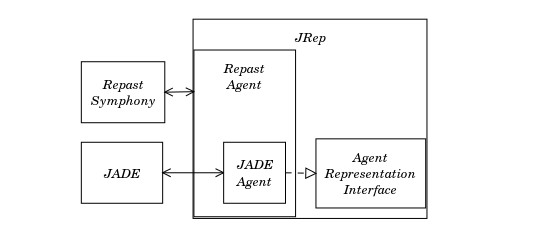
\includegraphics[width=0.5\textwidth]{figures/jrep.png}
	\caption{Basic structure of JRep. Diagram
		adapted from original paper. \cite{garcia2011misia}}
	\label{fig:jrep}
\end{figure}

The most obvious advantage of the approach proposed in this paper is the possibility of using Repast interaction protocols without the need to interface with JADE.

JADE is a very rich platform, but for many simulation scenarios, the overhead introduce by it will have an impact on the simulation performance. \cite{mengistu2008scalability} \apiname{}, as we describe with more detail in the next section, uses an implementation of those protocols that is conceptually very close to JADE's but tailored for Repast with no extra dependencies - in fact, the API could be used with other frameworks with little adaptation.

As suggested by Figure \ref{fig:related-repacl}, \apiname{}'s general structure is simpler than that of JRep and MISIA because, while these take advantage of both frameworks' features, \apiname{} is focused on the interaction protocols. Furthermore, unlike those, our proposal does not force the dual representation of agents in both frameworks.

\begin{figure}[h]
	\centering
	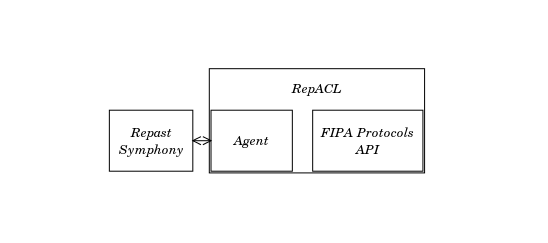
\includegraphics[width=0.5\textwidth]{figures/repacl.png}
	\caption{Basic structure of \apiname{} API}
	\label{fig:related-repacl}
\end{figure}

%!TEX root = doc.tex
\section{FIPA Specifications} % (fold)
\label{sec:fipa}

% Intro to FIPA in JADE/API
\apiname{} closely follows JADE's architecture regarding the use of protocols and services specified by \gls{FIPA}. The architecture of the API described in this paper includes multiple concepts proposed by \gls{FIPA}: the \gls{DF}, the \gls{MTS}, the \gls{AMS}, the \gls{ACL} Message and the Interaction Protocols. The following is a brief description of these concepts and of how JADE uses and implements them.

%\begin{figure}
%	\centering
%	\includegraphics[width=2.5in]{figures/pdf/AMSdiagram.pdf}
%	\caption{
%		Agent Management Reference Model, as specified by FIPA and implemented by JADE. \apiname{} only supports a single Agent Platform.
%	}
%	\label{fig:AMSdiagram}
%\end{figure}

% DF 
The \gls{DF} is a component that provides a yellow page service and is part of the FIPA Agent Management Specification. It allows one agent to perform searches about agents rendering specific services. Only agents that are registered in the DF will be indexed and agents can register and deregister themselves at any time.

% DF Agent Description
When searching the DF, agents can use templates that filter the search results. A DF Agent Description represents this template and contains the fields listed in Table \ref{tab:dfAgentDescription}.

\begin{table}
	\normalsize
	\caption{Fields of the DF Agent Description used to filter results of the DF service.}
	\label{tab:dfAgentDescription}
	\begin{center}
		\begin{tabular}{c|c}
		\hline
		\textbf{Parameter} & \textbf{Description} \\
		\hline
		\texttt{name} & The identifier of the agent \\
		\hline
		\texttt{services} & A list of services supported by this agent \\
		\hline
		\texttt{protocol} & A list of interaction protocols supported by the agent. \\
		\hline
		\texttt{ontology} & A list of ontologies known by the agent. \\
		\hline
		\texttt{language} & A list of content languages known by the agent. \\
		\hline
		\end{tabular}
	\end{center}
\end{table} 

% MTS
The \gls{MTS} is a service for transportation of ACL messages between agents. It is responsible for resolving agent addresses, in order to be able to deliver those messages. The MTS may request information from the DF or the AMS to perform this address resolution.

% AMS
The AMS is a mandatory component in FIPA-compliant agent platforms. Its purpose is to manage the agent platform, namely the creating and deletion of agents.

% ACL Message
The ACL Message is the envelope that contains the details for communication. \gls{ACL} stipulates what fields a message should contain. Table \ref{tab:fipaACLMessage} was adapted from the FIPA ACL Message structure specification and contains the list of fields in a message. Not all of them are mandatory. FIPA specifies the \texttt{performative} as the only mandatory field, although the \texttt{sender}, \texttt{receiver} and \texttt{content} are expected to be present.

\begin{table}
	\normalsize
	\caption{FIPA ACL Message Parameters. The highlighted fields are the ones featured in the current version of \apiname{}.}
	\label{tab:fipaACLMessage}
	\begin{center}
		\fboxsep1pt
		\begin{tabular}{c|c}
		\hline
		\textbf{Parameter} & \textbf{Category of Parameters} \\
		\hline
		\colorbox{Apricot}{\texttt{performative}} & Type of communicative acts \\
		\hline
		\colorbox{Apricot}{\texttt{sender}} & \multirow{3}{*}{Participant in communication} \\
		\cline{1-1}
		\colorbox{Apricot}{\texttt{receiver}} \\
		\cline{1-1}
		\texttt{reply-to}  \\
		\hline
		\colorbox{Apricot}{\texttt{content}} & Content of message \\
		\hline
		\texttt{language} & \multirow{3}{*}{Description of Content} \\
		\cline{1-1}
		\texttt{encoding} \\
		\cline{1-1}
		\colorbox{Apricot}{\texttt{ontology}} \\
		\hline
		\colorbox{Apricot}{\texttt{protocol}} & \multirow{5}{*}{Control of conversation} \\
		\cline{1-1}
		\colorbox{Apricot}{\texttt{conversation-id}} \\
		\cline{1-1}
		\texttt{reply-with} \\
		\cline{1-1}
		\texttt{in-reply-to} \\
		\cline{1-1}
		\colorbox{Apricot}{\texttt{reply-by}} \\
		\hline
		\end{tabular}
	\end{center}
\end{table} 

% Protocols In FIPA
FIPA Interaction Protocols typify communication interactions among agents by specifying two roles: initiator (the agent starting the interaction) and responder (a participant in the interaction). Each protocol defines precisely which messages are sent by each role ad in which sequence.

% Behaviors in JADE
In JADE, every agent activity is programmed through the notion o behaviours. For interaction protocols, typically behaviour-pairs are used for each side of the interaction, and JADE's API supports the most important protocols with built-in initiator and responder behaviours.
% Implementing these protocols.
In order to create an application using these protocols, programmers only need to extend these behaviours and implement the message handlers.
All the complexity regarding the interaction and networking infrastructure is hidden and taken care of by JADE, allowing the programmer to focus on the implementation of agent behaviour.
%!TEX root = doc.tex
\section{The \apiname{} API} % (fold)
\label{sec:proposal}

At times, when developing MAS on a specific platform, a need arises for adopting different tools than those available in the original platform. More specifically, this paper is the result of a necessity to quickly and easily create JADE-based applications out of Repast-based simulations, eventually being able to perform the complementary operation. \apiname{}'s main goal is to enable in Repast the support for the development of FIPA-compliant MABS. In this section we try to give a thorough description of \apiname{}'s architecture while comparing our design decisions with those of JADE.
% [citation needed: is conversion a real need?]

\subsection{Repast and JADE}
% What was missing in Repast?
JADE and Repast are two popular agent-based application development tools with a very distinct set of features. Table \ref{tab:jadevsrep} summarizes the main differences between the two. It's worth pointing out that communication and ontologies are both covered by FIPA specifications. This, together with the differences in agent execution, make up the targets of out API.

Our goal is not to reproduce JADE's distribution architecture in Repast. One advantage of using Repast is that, since the communication is local (while JADE's agents are often spread in different containers), the execution of Repast-based simulations is typically much faster. This also makes it more suited to perform simulations and tests on MAS \cite{mengistu2008scalability} \cite{gormer2011jrep} \cite{garcia2011misia}.

By incorporating FIPA specifications in Repast, we bring it closer to JADE. By using \apiname{}, programmers that are already comfortable with creating MAS in JADE can feel comfortable enough to produce Repast-based simulations with the tools they're used to in JADE.

\begin{table}[h]
	\normalsize
	\caption{Summary of JADE and Repast features.}
	\label{tab:jadevsrep}
	\begin{center}
		\begin{tabular}{l|cc}
		\hline

		\hline
		\textbf{} & \textbf{JADE} & \textbf{Repast} \\ %& \textbf{Cougaar} \\
		\hline
			Agent 		& FIPA  	&  Method calls  \\ %& Serialized Object \\
			Interaction	& protocols	&  Shared resources \\
		\hline
			Distribution & Yes & No \\ %& Yes \\
		\hline
			Simulation Tools & No & Yes \\ %& Yes \\
		\hline
			Scalability & Limited & High \\ %& High \\
		\hline
			Ontologies & Yes & No \\ %& Yes\\
		\hline
			Open Source & Yes & Yes \\ %& Yes\\
		\hline
			Agent  		& Behavior-based & Schedule-based  \\ %&  \\
			Execution	& Multi-threaded & Single-threaded \\ %&  \\
						& Event-driven   & Tick-driven 	   \\ %&  \\
						& Assync		 & Sync 		   \\ %&  \\
		\hline
		\end{tabular}
	\end{center}
\end{table} 

\subsection{FIPA Specifications}

As mentioned before, \apiname{} closely follows JADE's architecture regarding the use of protocols and services specified by FIPA. The architecture described in this paper includes four main concepts proposed by FIPA: the Directory Facilitator (DF), the Message Transport Service (MTS), the ACL Message and the Interaction protocols.

The DF is a component that provides a yellow page service and is part FIPA Agent Management Specification \footnote{FIPA AM - http://www.fipa.org/specs/fipa00023/XC00023H.html}. It allows one agent to perform searches in order to request information about other agents. Only agents that are registered in the DF will be indexed and agents can register and deregister themselves at any time. These searches can be filtered in order to find the agents that are announcing themselves as providers or certain service. 

In \apiname{}, the services used as filters in search are the type of interaction behavior that an agent is expected to have adopted. Since the context of out tool is the development local (vs. distributed) simulations, a single DF exists in each simulation. Is worth noting that Repast has it's own agent manager, named ``Context''. \apiname{} offers support to this feature by integrating a reference to this object in the DF.

The MTS is a service, also specified by FIPA \footnote{FIPA MTS - http://www.fipa.org/specs/fipa00067/SC00067F.html}, for transportation of ACL messages between agents. One of its tasks is to be able to resolve agent addresses, in order to be able to deliver those messages. \apiname{}'s implementation of the MTS is simplified. Since \apiname{}'s target is the development of simulations in Repast, all our agents are local and agent address resolution is not required.

The ACL Message is the envelope that contains the details for communication. ACL (Agent Communication Language) is specified by FIPA, which stipulates what fields the message should contain. Table \ref{tab:fipaACLMessage} was adapted from the FIPA ACL Message structure specification and gives and contains the list of fields in a message. Not all of them are mandatory. FIPA specifies the \texttt{performative} as the only mandatory field, although the \texttt{sender}, \texttt{receiver} and \texttt{content} are usually expected to be present.\footnote{http://www.fipa.org/specs/fipa00061/SC00061G.html}.

Our implementation uses a version of the ACL Message that is slightly simpler than in the one found in JADE. The language, encoding and reply-by fields were omitted in the current version. Also, the ontology field is simply a text field. \apiname{} does not support more complex ontologies at present time.

\begin{table}[h]
	\normalsize
	\caption{FIPA ACL Message Parameters}
	\label{tab:fipaACLMessage}
	\begin{center}
		\begin{tabular}{cc}
		\hline
		\textbf{Parameter} & \textbf{Category of Parameters} \\
		\hline
		\texttt{performative} & Type of communicative acts \\
		\hline
		\texttt{sender} & Participant in communication \\
		\hline
		\texttt{receiver} & Participant in communication \\
		\hline
		\texttt{reply-to} & Participant in communication \\
		\hline
		\texttt{content} & Content of message \\
		\hline
		\texttt{language} & Description of Content \\
		\hline
		\texttt{encoding} & Description of Content \\
		\hline
		\texttt{ontology} & Description of Content \\
		\hline
		\texttt{protocol} & Control of conversation \\
		\hline
		\texttt{conversation-id} & Control of conversation \\
		\hline
		\texttt{reply-with} & Control of conversation \\
		\hline
		\texttt{in-reply-to} & Control of conversation \\
		\hline
		\texttt{reply-by} & Control of conversation \\
		\end{tabular}
	\end{center}
\end{table} 

Finally, the main focus of the software we're proposing is the incorporation of FIPA Interaction Protocols in Repast. At the present time, we chose to include a few of the most common protocols in \apiname{}, following JADE's implementation.

The FIPA protocols from JADE we chose to include in \apiname{} at this point were the ``request-like'' Achieve Rational Effect (AchieveRE) protocol, the Propose protocol and the Contract Net protocol. The AchieveRE is a single protocol that encompasses multiple FIPA protocols, namely FIPA-Request, FIPA-query, FIPA-Request-When, FIPA-recruiting and FIPA-brokering protocols, as defined in JADE's documentation \footnote{http://jade.tilab.com/doc/api/jade/proto/AchieveREInitiator.html}.



\subsection{Agent Execution}

In the process of incorporating FIPA specifications, there was a necessity to make adaptations to JADE's protocols to

to reproduce Repast's the concept of time in JADE's protocols, which are essentially event-driven. In \apiname{}, communication happens asynchronously but not event-driven. As Figures \ref{fig:com-example-jade} and \ref{fig:com-example-repast} try to illustrate, agent execution in JADE and \apiname{} are significantly different.

Agent execution in Repast in not concurrent. Repast uses a time-share type of execution, granting each agent the right to perform its tasks until they finish them, in sequence, but in no particular order. Figure \ref{fig:com-example-repast} represents a best case scenario where the order of execution of the agents by Repast was favorable to communication. It's not unexpected for Agents A and B to execute again once before Agent C does, making the protocol take a bit longer to finish.

JADE agent execution, on the other hand, is concurrent and possibly parallel, since JADE supports distributed and multi-threaded agent systems.

\begin{figure}[h]
	\centering
	\includegraphics[width=3.0in]{figures/tickExample2.pdf}
	\caption{
		Communication example in JADE. Agents are executed concurrently or in parallel. Agent C tries to handle messages as they arrive and issues the respective reply.
	}
	\label{fig:com-example-jade}
\end{figure}

\begin{figure}[h]
	\centering
	\includegraphics[width=3.5in]{figures/tickExample.pdf}
	\caption{
		Communication example in Repast using \apiname{} in a single tick. In their respective turns, A and B send a message to C, which stays in standby in C's Mailbox. Only in C's turn do these messages get handled.
	}
	\label{fig:com-example-repast}
\end{figure}

Our approach when adapting Jade-based protocols was to use a mail box for each agent. Messages in the mail box will not be processed until Repast grants execution to the behaviors whose agent owns that mail box. It's worth noting that the order by which Repast executes each scheduled item is never guaranteed. In fact, it's not guaranteed that all the behaviors or a single agent are executed together. This is the expected behavior when working with Repast as well as with JADE and it is up to the programmer to ensure that the application does not depend on the order or execution.

\subsection{Architecture}

Figure \ref{fig:arch} illustrates the details of \apiname{}'s architecture. Most concepts represented in this diagram are present in JADE, namely the Agent, ACL Message, Behavior, MTS and DF service.

As mentioned before, an agent in \apiname{} contains a queue of Behaviors and a mail box. On each ``round'', these behaviors are schedules to be executed and some will take care of handling the messages arrived at the mail box.

The protocol package contains the implementation of the different FIPA protocols. Other protocols can be created by extending these and creating new behaviors can be done by extending the main Behavior. The typical work flow when developing a new protocol, is to select the most appropriate one among the one available and implement a set of handlers for the ACL Messages. These handlers are called at certain states of the protocol and all the protocol logic is perform in the backstage.

The ACL message, the DF and the MF shown in Figure \ref{fig:arch} are described with more detail in the previous section about FIPA Specifications.

\begin{figure}[h]
	\centering
	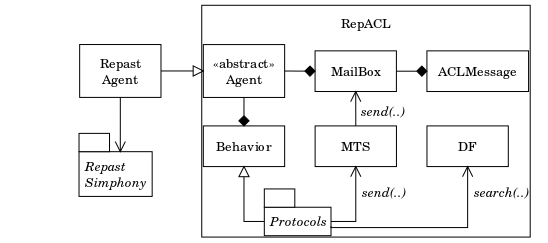
\includegraphics[width=3.5in]{figures/repacl_arch.pdf}
	\caption{Detailed architecture or \apiname{}}
	\label{fig:arch}
\end{figure}



% section proposal (end)
%!TEX root = doc.tex
\section{Validation}
\label{sec:verification}

To perform a validation of the API, we developed a contract net scenario. This is a deterministic test which uses a fixed data set, thus having always the same outcome. The example was implemented in Repast (using \apiname{}) and then manually ported to JADE, after some adaptations.

\subsection{Experimental Setup}

The diagram in Figure \ref{fig:CNetExample} illustrates the contract net created for this test. An agent (the buyer) intends to purchase a certain quantity of three kinds of goods: rice, flour and oats. Besides the quantities of each product it needs, the buyer also stipulates a maximum price for the whole deal. The buyer will issue a call for proposals (CFP) containing a request for supplies to all agents that announce themselves as suppliers in the DF.

Supplier agents have a maximum supply capacity and a price for each product. After receiving a CFP, the supplier will send to the buyer a PROPOSAL containing a price for each product if the demanded supply is within the seller's capacity. Otherwise, a REFUSE message will be sent to the buyer.
Finally, the buyer agent will compare all valid proposals, choose the cheapest offer for each individual product and reply with an ACCEPT PROPOSAL to the best offers, and REJECT PROPOSAL to all others.

\begin{figure}
	\centering
	\includegraphics[width=3.0in]{figures/CNetExample.pdf}
	\caption{
		Representation of the example contract net.
	}
	\label{fig:CNetExample}
\end{figure}

Using the same data set with values for prices and supply capacity in both frameworks, we ensured the proper comparison of results. For demonstration purposes, we focused on two simple metrics to evaluate our work: time and outcome. We have run the same experiment with varying numbers of suppliers (as sugested by Figure \ref{fig:performance}) and performed multiple repetitions of each setup.

Time was measured from be begining of the protocol, until all suppliers were notified. The JADE implementation was tested in two different setups: first, with all agents running in a single container; second, with the supplier agents in one container and the buyer in a separate one (but in the same host). In this configuration, all communication between agents happens across containers. All tests were performed using an Intel i7 CPU with 8 logical cores at 2.20 GHz. The second validation metric we used was the actual result of the protocol, i.e who were the supplier agents chosen by the buyer and their price proposals.

\subsection{Results}

For each number of agents, the experiment was run 5 times. The average performance of the experiments is represented in Figure \ref{fig:performance}. As excepted, Repast performance was significantly better, and it excels when the number of agents is high. JADE was able to perform better when using two distinct containers. As studied by Mengistu et. al \cite{mengistu2008scalability}, JADE's performance drops very significantly when there is a high communication-to-computation ratio in the application.

Regarding the outcome of the protocol, as expected the same values were obtained in both implementations, with equal number of suppliers. This allowed us to verify that the behaviour of the protocol is identical in both implementations.


%%%%%%%%%%%%%%%%%%%%%%%%%%%%%%%%%%%%%%%%%%%%%%%
%%%%%%%%%%%%%%%%%% The Chart %%%%%%%%%%%%%%%%%%

\begin{figure}
	\label{fig:performance}
	\centering
	%\includegraphics[width=\linewidth]{figures/performance.png}
	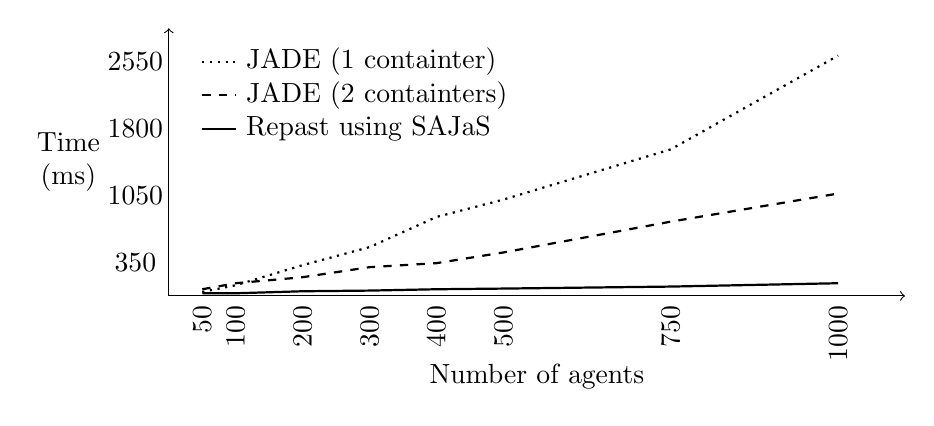
\begin{tikzpicture}[scale=0.85]

		% horizontal axis
		\draw[->] (0,0) -- (11,0);
		\draw (5.5,-1.2) node[align=center] {Number of agents}; %label

		%					  north
		%			west [anchor center] east
		%					  south
		
		% labels
		\draw	(0.5,0) node[rotate=90, anchor=east] {50}
				(1.0,0) node[rotate=90, anchor=east] {100}
				(2.0,0) node[rotate=90, anchor=east] {200}
				(3.0,0) node[rotate=90, anchor=east] {300}
				(4.0,0) node[rotate=90, anchor=east] {400}
				(5.0,0) node[rotate=90, anchor=east] {500}
				(7.5,0) node[rotate=90, anchor=east] {750}
				(10.,0) node[rotate=90, anchor=east] {1000};

		\draw	(-0.5,0.5) node[anchor=center] {350}
				(-0.5,1.5) node[anchor=center] {1050}
				(-0.5,2.5) node[anchor=center] {1800}
				(-0.5,3.5) node[anchor=center] {2550};
		% vertical axis
		\draw[->] (0,0) -- (0,4);
		\draw (-1.5,2) node[align=center] {Time\\(ms)}; %label
		%\draw (-1.5,1.6) node[align=center] {(ms)}; %label

		%% Data %%
		% JADE 2 containers
		\draw[thick,dashed] (0.5,3.0) --
			(1,3.0) node[anchor=west, pos=1.0] {JADE (2 containters)}; %subtitle
		\draw[thick,dashed] (0.5, 0.10) --
					(1.0, 0.19) --
					(2.0, 0.28) --
					(3.0, 0.43) --
					(4.0, 0.49) --
					(5.0, 0.65) --
					(7.5, 1.11) --
					(10., 1.53);
		% JADE 1 containers
		\draw[thick,dotted] (0.5,3.5) --
			(1,3.5) node[anchor=west, pos=1.0] {JADE (1 containter)}; %subtitle
		\draw[thick,dotted] (0.5, 0.06) --
					(1.0, 0.16) --
					(2.0, 0.46) --
					(3.0, 0.73) --
					(4.0, 1.18) --
					(5.0, 1.44) --
					(7.5, 2.19) --
					(10., 3.59);
		% Repast
		\draw[thick] (0.5,2.5) --
			(1,2.5) node[anchor=west, pos=1.0] {Repast using \apiname{}}; %subtitle
		\draw[thick] (0.5, 0.04) --
					(1.0, 0.04) --
					(2.0, 0.07) --
					(3.0, 0.08) --
					(4.0, 0.10) --
					(5.0, 0.11) --
					(7.5, 0.14) --
					(10., 0.19);


	\end{tikzpicture}
	\caption{
		Average execution time of each framework in the different experiments.
	}
\end{figure}

%%%%%%%%%%%%%%%%%%%%%%%%%%%%%%%%%%%%%%%%%%%%%%%
%%%%%%%%%%%%%%%%%%%%%%%%%%%%%%%%%%%%%%%%%%%%%%%

%!TEX root = doc.tex
\section{Future Work}
\label{sec:prototype}

In this section we specify some of the future developments that are planned for \apiname. We also present the tool under development that initially created the need for the development of \apiname.

\subsection{Conversion Tool Prototype}

The goal of the tool we propose is to allow the automatic conversion of Repast simulations into JADE applications. This conversion tool will not only allow the developer to quickly generate a MAS or create a simulation but also enables a proficient programmer in one framework to quickly get started in developing with the other framework. Figure \ref{fig:prototypeFlow} illustrates these two plausible workflows.

\begin{figure}[h]
	\centering
	\includegraphics[width=3.0in]{figures/prototypeFlow.pdf}
	\caption{
		Two possible workflows for \apiname{} users
	}
	\label{fig:prototypeFlow}
\end{figure}

The code conversion tool uses the Java Development Tools (JDT) from Eclipse which enables Java programmers to perform introspection and reflection tasks with ease. This approach allows programmers to perform code transformations without having to create parsers for Java code and abstract syntax trees (AST).

The conversion tool will be developed in the form of an Eclipse plug-in, in order to be able to make use of all JDT features.

\subsection{\apiname{} development}

Although \apiname{} is already fit for development of Repast simulations, it's still an ongoing project. One important trait of \apiname{} is that, although tailored for repast, it's very generic. This means that MABS built using other Java simulation tools can integrate our API successfully in the future and, therefore, use Jade-based tools.

%!TEX root = .\doc.tex
\section{Conclusion}
\label{sec:conclusion}

The development of MAS may require the use of tools that are not readily available in the agent-based framework originally chosen. The API architecture we propose in this paper emerges as a need to solve a concrete instance of this problem. \apiname{} is our solution to integrating FIPA specifications in MABS frameworks, more specifically Repast, as well as allowing the creation of JADE-based simulations.

The goal of our API is not only to enrich Repast and other simulation frameworks, but also to allow proficient JADE developers in quickly getting started in developing simulations using familiar JADE-based tools. \apiname{} also opens the door to MAS to MABS conversion.

The short experiment we described in the previous section showed that our API is capable of handling simulations with a large number of agents, which is common in many simulation scenarios. Aside from the inherent advantages of using open standards in agent systems, \apiname{}'s JADE-based architecture brings Repast closer to JADE. The immediate result of this architecture is that converting models built with Repast using \apiname{} into JADE MAS is very straightforward.


%\bibliographystyle{llncs}
%\bibliography{IEEEabrv, references}
%\bibliographystyle{splncs}
%\bibliographystyle{spbasic}
\bibliographystyle{plain}
\bibliography{references}


\end{document}

